\chapter{Projektbeskrivelse}
\section{Projektgennemførelse}
 
Dette projekt er gennemført vha. forskellige udviklingsprocessor, hvilket er med til at sikre kvalitet, og at deadlines overholdes. En af disse modeller er ASE-modellen \cite{ISE}. Denne model er en udviklingsmodel, der er udarbejdet af Aarhus Ingeniørhøjskole. Modellen er en gentagelig udviklingsproces drevet ud fra projektets Use Cases. Modellen er benyttet på den måde, at gruppemedlemmerne fastlægger en projektformulering, kravspecifikation og systemarkitektur, for derefter at designe og implementere de enkelte hardware- og softwaredele. Gennem en integrationstest ses det om hardware- og softwaredelene fungere som de skal.  
Dette ender med en gennemført accepttest, således at det testes om systemet lever op til kravene.
\begin{figure}[H]
	\centering
	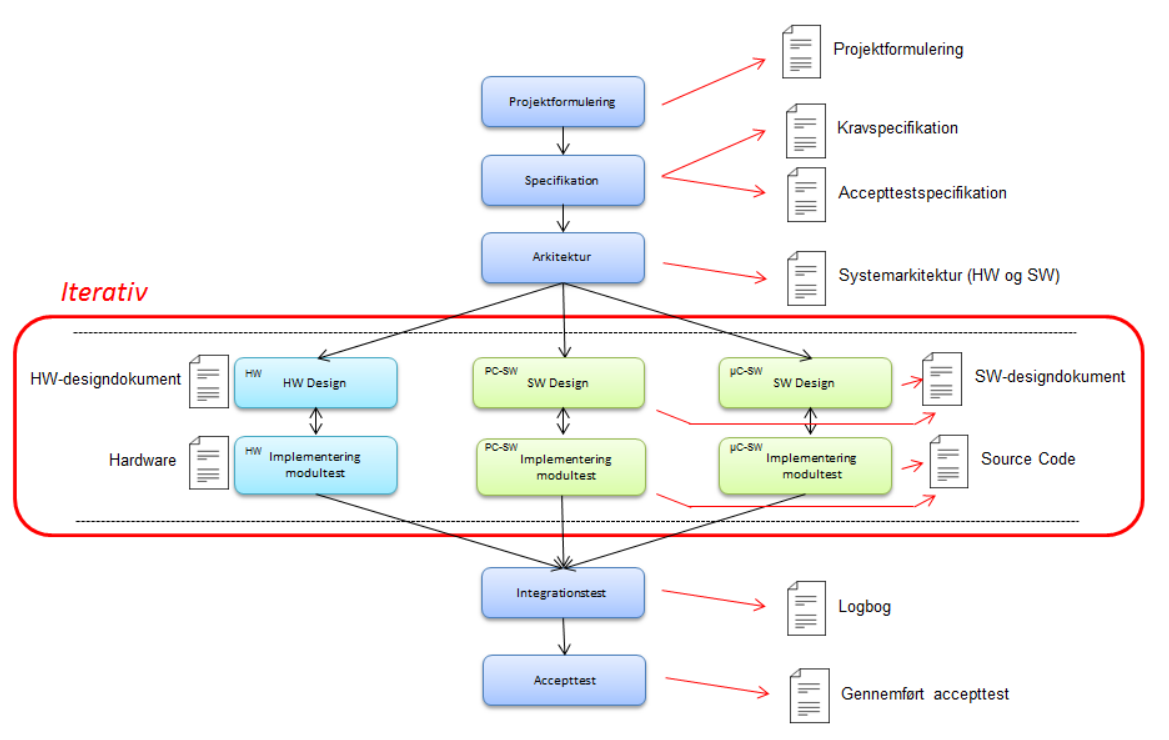
\includegraphics[width=0.8\textwidth]{Figurer/AseModellen}
	\caption{ASE-modellen}
	\label{fig:ASE_model}
\end{figure}
For at forstå ASE-modellen \cite{ISE} er det vigtigt at gennemgå Use Cases; et værktøj, som skal beskrive interaktioner mellem diverse aktører og selve systemet. Sammen med de ikke-funktionelle krav opnås et overblik over hvilke funktionalitetskrav, der stilles til systemet. På baggrund af kravspecifikationen kan accepttesten efterfølgende udarbejdes. I dette projekt er hardware- og software design implementering på lige fod, da projektet består af begge ting ligeligt.\\
\newline
V-modellen \cite{ISE} er en faseopdelt udviklingsmodel, der også er værd at nævne i dette projekt. Den beskriver udviklingsfaserne og testfaserne sideløbende i forhold til projektet, og den er derfor benyttet til dette projekt sideløbende med ASE-modellen. Modellen fungerer således, at specifikationen af test foregår parallelt med udviklingen af selve systemet.

\begin{figure}[H]
	\centering
	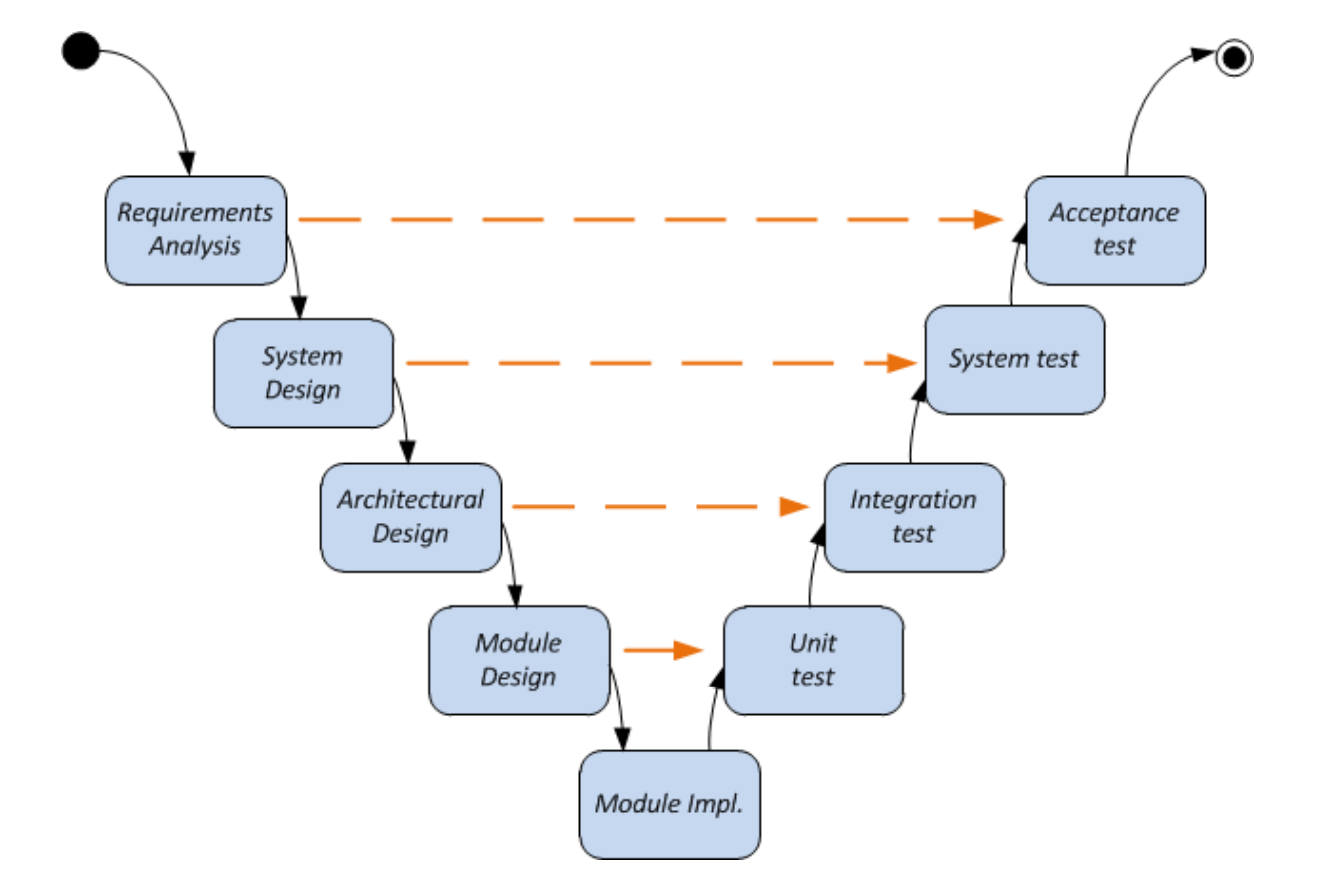
\includegraphics[width=0.6\textwidth]{Figurer/VModellen}
	\caption{V-model}
	\label{fig:V_Modellen}
\end{figure}

Den er blevet benyttet til hardware- og softwareudviklingen. Hardware og software skulle begge teste deres funktioner inden nye faser blev igangsat, for at verificere om disse funktioner virkede korrekt gennem forløbet. Fordelen ved at teste på forskellige niveauer er, at det skal sikre de udviklede delsystemer, således at de virker som planlagt. Det er vigtigt, at hver fase er udført, før den næste fase påbegyndes. 
\newline

Vandfaldsmodellen \cite{ISE} er også benyttet under dette projekt. Softwareudviklingen bærer præg af vandfaldsmodellen, da udviklingen er opdelt i faser, hvor hver fase er blevet gennemført, før den næste er påbegyndt. Dette er i relation til V-modellen, som blev beskrevet før og den er konstant strømmende nedad. 

\begin{figure}[H]
	\centering
	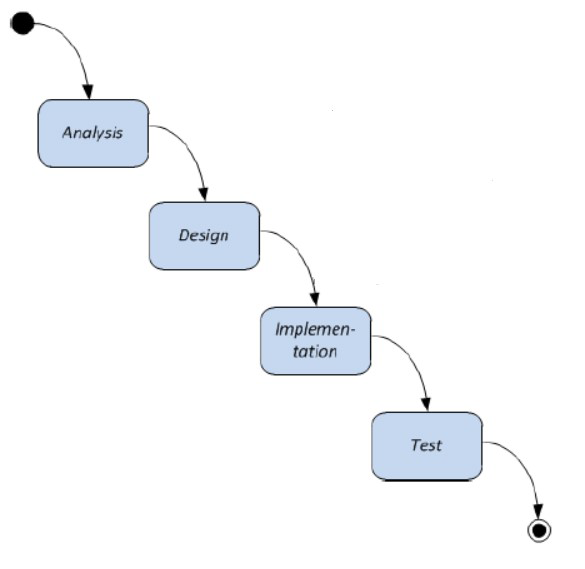
\includegraphics[width=0.4\textwidth]{Figurer/VandfaldsModellen}
	\caption{Vandfalds modellen}
	\label{fig:vandfalds_model}
\end{figure}


\section{Projektstyring}
Projektet er udarbejdet over et semester, hvor undervisningen og forelæsningerne delvist har udgjort grundlaget for teorien benyttet i projekt. Der blev i starten udarbejdet en tidsplan med enkelte faste deadlines og med mulighed for at sætte andre deadlines løbende i processen. Se Tidsplan under Bilag.\\ 
Projektgruppen har bestået af 6 gruppemedlemmer, som er blevet delt i to fokusområder, hardware og software. Fordelingen blev udarbejdet efter den enkeltes ønske. Projektet  har  været afhængig af, at der var god kommunikation mellem de to undergrupper.
Da gruppen har været opdelt, har der været projektmøde hver uge, hvor gruppen har opdateret hinanden og vejleder. Samtidigt har gruppen forsøgt at sidde samlet, så på den måde at kunne opdatere hinanden løbende.\\
Under projektet har alle medlemmer været med til, at sikre en administrativ kæde af deadlines til individuelle opgaver, samt dagsordener til hvert møde. Disse deadlines har sikret at opgaverne er blevet opfyldt op til møderne og det har derfor været nemt at følge op på. Da der har været overlap mellem forskellige opgaver er der løbende blevet kørt og lavet adskillige teste for at sikre at opgaverne har været vellykket.  
 

\section{Metoder}
Til at kunne overskue arkitektur og designet af projektet, er flere forskellige arbejdsmetoder benyttet for at skabe det bedst mulige resultat. 
For at finde, hvad blodtryksmåleren skal gøre, er der blevet udarbejdet Use Cases. Disse beskriver systemet funktionalitet. Use Cases viser, hvad brugeren skal opleve fra systemet, men ikke, hvordan det sker. I Use Case diagrammet bliver det også vist, hvilke aktører der findes og hvordan de interagerer med systemet.   \\
I projektet bruges accepttest til at teste blodtryksmåleren. Dette gøres ud fra kravspecifikationen, hvor det er angivet, hvilke krav der er stillet til systemet. \\Accepttesten er en test, hvor der beskrives, hvad der skal ske og, hvad brugeren skal gøre. Testen er for at undersøge om produktet opfylder de krav, der er blevet sat for det. Accepttesten giver et godt overblik for udvikleren og for kunden, der nemt og hurtigt kan se om produktet virker som det skal. \\
\newline
Til  beskrivelse af design af software og hardware er diagrammer og skemaer blevet udarbejdet i SysML og UML. SysML er et grafisk modelleringssprog, som kan bruges til at overskueliggøre systemer. \\
Til software er der blandt andet lavet en applikationsmodel i SysML, som består af et domæne-, klasse- og sekvensdiagram. \\
Domænemodellen viser sammenhængen mellem blokkene i systemet. Blokkene findes i Use Casene og derved bliver disse to ting koblet sammen. \\
Klassediagrammet viser, hvilke metoder blokkene har og hvordan de kommunikerer med hinanden. Her findes domæne-, kontrol- og grænsefladeklasser. Kontrolklasserne beskriver, hvordan data behandles mellem domæne- og grænsefladeklasser. Domæneklasser indeholder funktionalitet fra den pågældende softwareblok. Grænsefladeklasserne viser, hvordan, systemet interagerer med omverdenen. Diagrammet gør det nemmere at fremme en lav kobling og høj samhørighed i softwaren.\\
Sekvensdiagrammet fortæller, hvad der sker i selve koden. Igen går det ud fra Use Casene, hvor vægten nu er på softwaredelen. Derved beskrives det, hvordan metoder bliver kaldt og hvordan de forskellige klasser interagerer. Hver Use Case skal her gennemgås i softwaren, så der skabes et overblik over vejen gennem koden.\\
\newline 
For at skabe et overblik og indsigt i koden, er der i UML udarbejdet et aktivitetsdiagram og et klassediagram. Aktivitetsdiagrammet går i dybden med en specifik metode. Det er kun blevet gjort for relevante metoder. Her tydeliggøres det, hvordan hver metode fungere og, hvad den indeholder.  Klassediagrammet fortæller hvilke metoder, en klasse indeholder og hvordan klasserne hænger sammen.\\
\newline  
Til hardwaren er der blevet brugt Block Definition Diagram(BDD), som viser hvilke blokke et system indeholder og hvilke porte de har. BDD er lavet til at give et overblik over systemet. Ud fra BDD’et er et Internal Block Diagram(IDB) blevet lavet. Her vises, hvilke signaler, som findes i systemet og hvordan de sendes rundt. Her vises portene igen og der skal være overensstemmelse mellem BDD og IBD.    
\newline 
Til udarbejdelsen af kredsløb blev Analog Discovery brugt til at simulerer signalet, som i sidste ende skal komme fra transduceren. Først blev kredsløbet opbygget på et fumlebræt, hvor det blev testet for at afprøve om det lever op til kravene. Når det opfylder kravene, flyttes det over på et Veroboard. Veroboardet bliver igen testet før aflevering. 

\section{Systemarkitektur}

\begin{figure}[H]
	\centering
	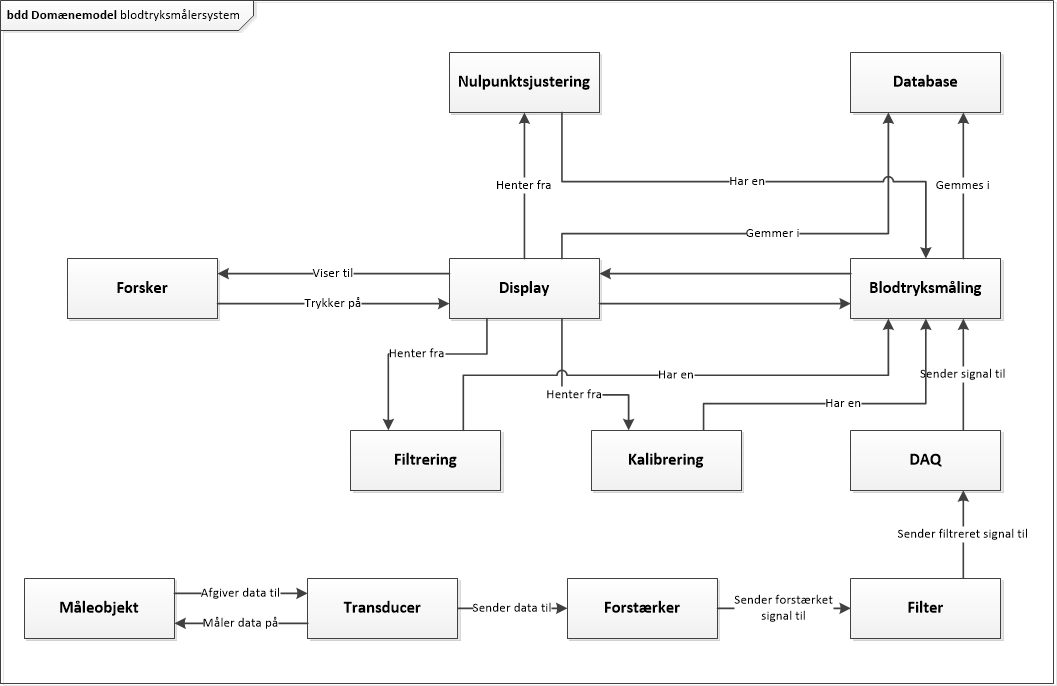
\includegraphics[width=1.0\textwidth]{Figurer/DomaneModel}
	\caption{Domæne Model}
	\label{fig:Domaene Model}
\end{figure}

\section{Hardware}
I hardwaredelen skal der ligge en forstærkning og et lavpasfilter. Det differentieret signal fra transduceren skal forstærkes og filtreres før det kan sendes ind i DAQ'en.

\subsection{Design)}
\subsubsection{Forstærkning}
Transduceren måler en trykændring, som den omsætter til en spænding. Dette er udtrykt ved et differentieret signal, som sendes ind i forstærker-blokken. \\
Signalet fra transduceren er en lav spænding, som skal forstærkes op, for at passe med DAQ'ens input. Denne forstærkning udregnes ud fra det maksimale output fra transduceren og det maksimale input til DAQ'en. Se beregningerne under implementering.  
\newline
Under simulering bruges Analog Discovery som en funktionsgenerator, der simulerer det differentieret signal.  

\subsubsection{Lavpas}
I projektet skal der laves et 2. ordens lavpasfilter. Filteret skal laves for at sikre, at der ikke opstår aliasering.\\
Aliasering \cite{DSB} er, hvor signalet bliver gentaget. Når man har signalet i det digitale domæne, bliver spektret for signalet en periodisk funktion.\\
Det skal sikres, at der ikke kommer overlap mellem signalet og et alias. Da det ellers kunne give anledning til misforståelser. Derfor laves et lavpasfilter, som sikre at der ikke ligger noget signal ved den halve samplingsfrekvens.\\
Lavpasfilteret skal være et Sallen-Key Butterworth-filter med en knækfrekvens på 50 Hz og en samplingsfrekvens på 1kHz. Ud fra oplysninger givet til projektet, vides det at filteret skal dæmpe signalet med 20 dB, under antagelse af at den forekommende støj er mindre end signalet, også når det forekommer over knækfrekvensen.\\
Ved en typisk blodtryksmåling forekommer der ikke signal over 50 Hz, samtidigt er signalet her aftaget med ca. 70 dB. For at få signalet, ved den halve samplingsfrekvens til at være $ 1/2 \cdot LSB $ (Least Significant Bit), skal det ydeligere dæmpes 20 dB. Derfor oplyses filteret til at være 50 Hz, da dette giver en minimum dæmpning på 20 dB pr. dekade.

\subsection{Implementering}
\subsubsection{Forstærkning}
For at få den rette forstærkning er det blevet valgt, at benytte instrumentationsforstærkeren INA-114. Her kan transduceren sættes på med det differentierede signal. INA-114 er valgt da følgende gælder\cite{Instrumentation} for instrumentationsforstærkere: 
\begin{itemize}
	\item Differentielt input - single ended output 
	\item Gain justering med ændring af kun én modstand 
	\item Meget høj indgangsimpedans 
	\item Stor Common Mode Rejection Ratio (CMRR)
\end{itemize}
For at udregne den korrekte forstærkning, bruges følsomheden fra transduceren og eksistationsspændingen.
Først udregnes det maksimale output fra transduceren:   
\begin{ceqn}
\begin{equation}
9V\cdot 250mmHg \cdot 5\mu\cdot 10^{-5} uV/V/mmHg  = 11.25mV
\end{equation} 
\end{ceqn}
Da det er besluttet at det maksimale input til DAQ'en \cite{DSB} er 5V, kan forstærkningen (Gain) nu udregnes:
\begin{ceqn}
\begin{equation}
\begin{split}
5V=& 11.25mV \cdot G \\
G =& 444.44
\end{split}
\end{equation}
\end{ceqn}
For at få den rette forstærkning udregnes den eksterne modstand ($ R_g $) til INA-114 \cite{INA}.\\ 
INA-114's forstærkning afhænger af størrelsen på $ R_g $, hvis modstanden er stor, er forstærkningen lille og omvendt.  $ R_g $ udregnes ved formlen: 
\begin{ceqn}
\begin{equation}
\begin{split}
G=&1+\frac{50k\Omega}{R_g}\\
444.44=& 1+\frac{50k\Omega}{R_g} \Rightarrow R_g= 112.75 \Omega
\end{split}
\end{equation}
\end{ceqn}
Derved fås en værdi for den eksterne modstand til INA-114, som skaber den ønskede forstærkning.\\
\newline
Den ønskede forstærkning kan bruges, da det passer over ens med båndbredden. Dette kan undersøges da produktet af forstærkning og båndbredde er konstant og båndbredden skal ligge over knækfrekvensen for filteret. Se beregning i Dokumentation ligning 3.4.\\
\newline 
For at imødekomme usikkerheden ved Analog Discovery, der bruger lave spændinger, laves et kredsløb efter spændingsdelerprincippet. Signalerne fra Analog Discovery skal sendes igennem dette kredsløb, hvor de efter spændingsdelerprincippet gøres mindre.\\  
Derved kan Analog Discovery sende signaler med en højere spænding ind i kredsløbet og usikkerheden mindskes. Hvis INA-114 skal have 11.25mV skal Analog Discovery sende 1.1352V ind.  
\\
\newline 
På figur \ref{fig:HW} ses et diagram af det endelige kredsløb med komponentværdier. Her ses, hvordan det ser ud ved realiseringen med transduceren og ved simuleringen ved Analog Discovery. 
\begin{figure}[H]
	\centering
	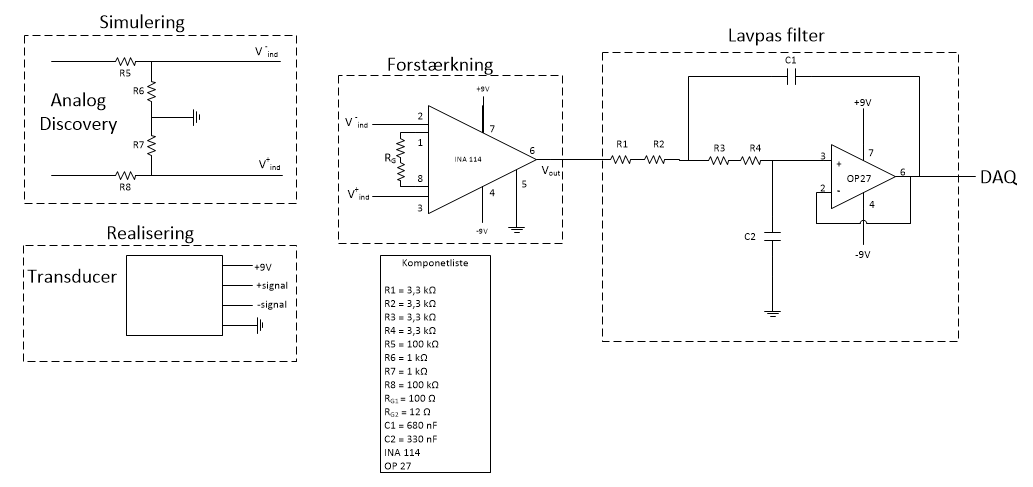
\includegraphics[width=1.0\textwidth]{Figurer/diagram_over_HW}
	\caption{Diagram over HW}
	\label{fig:HW}
\end{figure}

\subsubsection{Lavpas}
For at opnå den ønskede effekt i lavpasfilteret, blev det oplyst at $ f_c=50$ Hz, $ f_s = 1$kHz, $ R_1 = R_2 $ og $ C_2=680 nF$. Ud fra disse værdier, udregnes de resterende komponentværdier for filteret.

Overføringsfunktionen for et 2. ordens filter er:
\begin{ceqn} 
\begin{equation}
H(z)=\frac{\omega_n^2}{(s^2 + 2\cdot\zeta \cdot \omega_n \cdot s+\omega_n^2)}
\end{equation}
\end{ceqn}

For at finde overføringsfunktionen for det gældende system, vides det at følgende ligninger gælder \cite{Wikilavpas}:
\begin{ceqn}
\begin{equation}
\begin{split}
\omega_n = 2\cdot \pi\ 50 =& \dfrac{1}{\sqrt{R1\cdot R2\cdot C1\cdot C2}}\\
2\cdot \zeta\cdot\omega_n =&\frac{1}{C2}\cdot \left( \frac{R1+R2}{R1\cdot R2}\right)
\end{split}
\end{equation}
\end{ceqn}
Dette indsættes i den generelle overføringsfunktion og det simplificeres, blandt andet ved at det vides at $ R1=R2 $. 
Se Beregning af overføringsfunktion i Bilag for nærmere udregninger:
\begin{ceqn} 
\begin{equation}
H(z)=\dfrac{\dfrac{1}{C1 \cdot C2\cdot R^2}}{s^2+s\cdot \dfrac{2}{R\cdot C2}+ \dfrac{1}{C1\cdot C2\cdot R^2}}
\end{equation}
\end{ceqn}
Når der arbejdes med et 2. ordens Butterworth filter, vides det at udsvinget$ \zeta $ skal have værdien 0.7 \cite{ASB}.
Under beregningerne, var der usikkerhed omkring, hvad værdien af $ \zeta $ skulle være. Da kredsløbet skulle realiseres og dokumenteres blev det derfor overvejet at ændre samtlige komponentværdier så de passede med en $ \zeta = 1 $. Inden dette blev gjort blev det dokumenteret at det gælder at $ \zeta $ skal have en værdi på 0.7. \\
  
Den sidste overføringsfunktion sammenlignes med den generelle for 2. ordens systemer. Det gælder at $ C2 = 680\cdot 10^{-9} nF $. Det er så muligt at isolerer forskellige led. Først isoleres der for modstanden(midterste led i nævneren) og den udregnes til $ R = 6687\Omega $. \\
Nu kan det tredje led i nævner isoleres og kondensatoren $ C1 $ udregnes til $ C1 = 333 \cdot 10^{-9} nF $. \\
Nærmere beregninger kan ses under Systemarkitektur i Dokumentationen. \\
Alle komponentværdierne til lavpasfilteret er fundet og det kan nu realiseres. \\ 

Under udviklingen af lavpasfilteret er komponentstørrelserne, blevet ændret for at kunne realisere det. De brugte komponentværdier er: $ R= 6.6 k\Omega $, $ C1= 330\cdot 10 ^{-9} nF$ og $ C2= 680\cdot 10^{-9} nF$.   
For at være sikker på at filteret har de ønskede karakteristika, laves et bodeplot for den endelig overføringsfunktion: 
\begin{ceqn}
\begin{equation}
H(z)=\dfrac{62500000000}{610929\cdot \left( s^2+\dfrac{250000}{561}\cdot s + \dfrac{62500000000}{610929} \right)}
\end{equation}
\end{ceqn}
\begin{figure}[H]
	\centering
	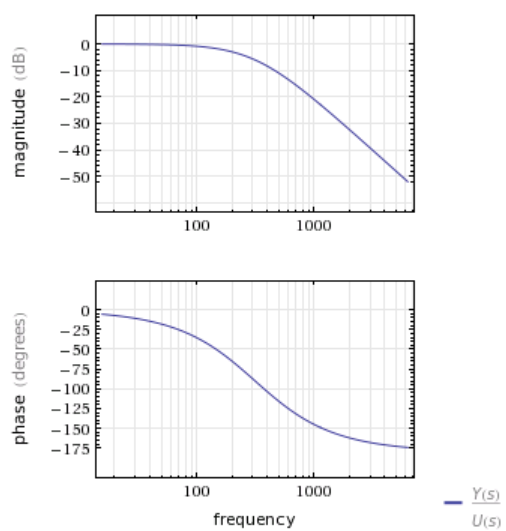
\includegraphics[width=0.5\textwidth]{Figurer/Bodeplot}
	\caption{Bodeplot}
	\label{fig:bodeplot}
\end{figure}
Ud fra den nye overføringsfunktion udregnes en nu $ \zeta $ for at kontrollere at værdien ikke har ændret sig. Denne udregnes til $ \zeta = 0.709 $. Derfor kan det konkluderes at filteret stadig har den ønskede funktionalitet. 

\subsection{Test}
\subsubsection{Forstærkning}
For at teste forstærkningen, sendes et differentieret signal ind vha. Analog Discovery. Her observeres der hvor meget signalet bliver forstærket. 
På figur \ref{fig:forstaerkning} ses det signal, som sendes ind i forstærkningsblokken og det, der måles på udgangen af blokken. 
\begin{figure}[H]
	\centering
	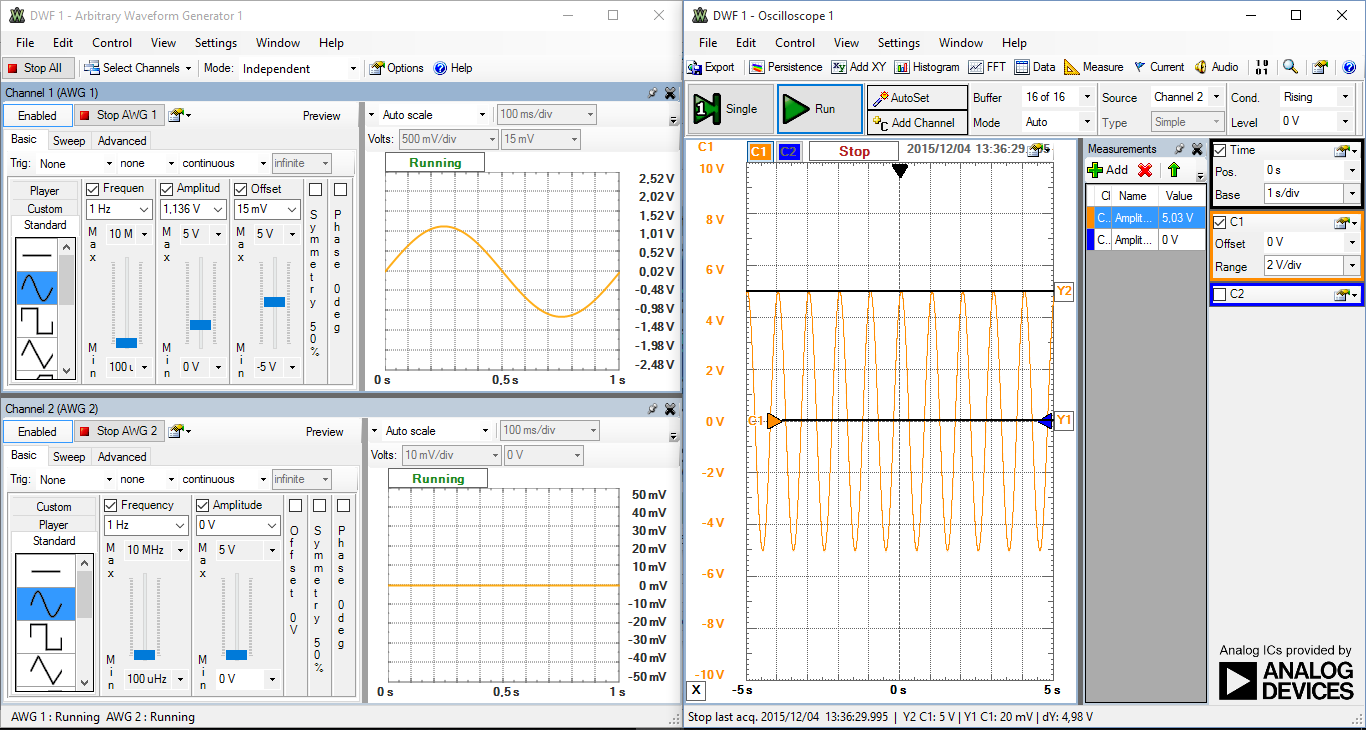
\includegraphics[width=1.0\textwidth]{Figurer/forst_blok}
	\caption{Forstærkningsblok}
	\label{fig:forstaerkning}
\end{figure}
Der sendes et differentieret signal ind i INA-114. På udgangen ses det at signalet er blevet forstærket op til 5V DC. Herved er maksimum input til forstærkningsblokken blevet forstærket så det passer med maksimum input til DAQ'en. Signalet bliver ikke ændret på andre måde i denne blok.

\subsubsection{Lavpas}
For at teste lavpasfilteret foretages målinger med en sinus, hvor frekvensen varierer for hver måling. Derved aflæses fasen mellem indgang- og udgangssignal, samt amplituden for hver måling. Der laves flere målinger, både før, ved og under knækfrekvensen. 
Ved knækfrekvensen skal fasedrejningen være 90\textdegree. Dette kan aflæses på figur \ref{fig:maeling50Hz}.\\
Se Modultest i Dokumentationen for mere dokumentation.  
\begin{figure}[H]
	\centering
	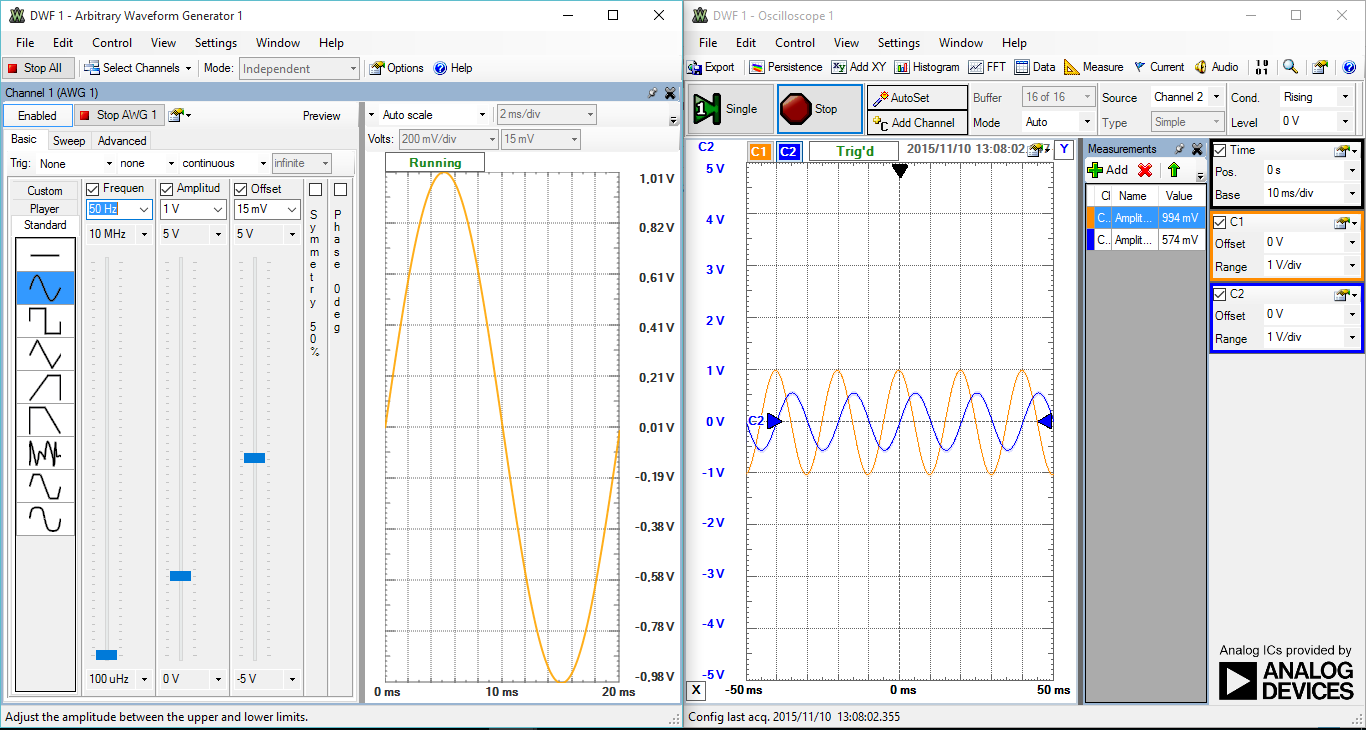
\includegraphics[width=1.0\textwidth]{Figurer/50Hz}
	\caption{Måling for 50 Hz}
	\label{fig:maeling50Hz}
\end{figure}


\subsubsection{Kalibrering med vandsøjle}
Efter forstærkning og lavpasfilteret er blevet testet hver for sig, udføres en kalibrering af systemet vha. en vandsøjle. Her bruges en udleveret vandsøjle med tre målepunkter, hvor det er angivet hvor højt trykket(målt i milimeter kviksølv, mmHg) er ved hvert af disse punkter. Derved kan det testes om hardwaredelen måler den rigtige spænding i forhold til mmHg. \\
Ud fra den maksimale spænding (målt i Volt, V) og mmHg kan det udregnes, hvad hardware skal vise ved 100 mmHg, se figur \ref{fig:graf_vandtest}. 
\begin{figure}[H]
	\centering
	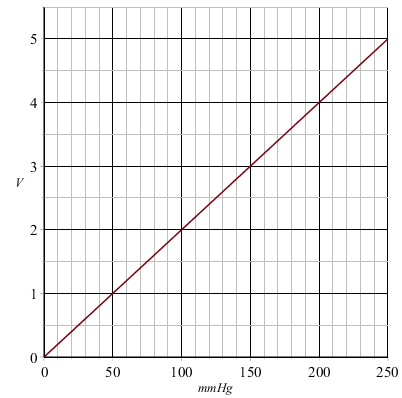
\includegraphics[width=0.3\textwidth]{Figurer/graf_vandtest}
	\caption{Graf til kalibrering, fra udregninger}
	\label{fig:graf_vandtest}
\end{figure}
Testen udføres ved at fylde vand i søjlen til et bestemt punkt. Transduceren skal være tilkoblet netop dette målepunkt, mens de andre er lukket til. Transduceren er sat til hardwaren, der hvor Analog Discovery tidligere har været sat til. Transduceren er tilkoblet 0-9V ved batterierne. På samme måde, som ved simuleringen, aflæses målingen på computeren ved hjælp af programmet WaveForms. Da det vides hvilken trykændring der måles på, ved vi fra grafen til kalibreringen hvilken spænding den skal vises. Dette fortages for de tre målepunkter på vandsøjlen, hvor hver måling sammenlignes med den udregnede graf. For hver måling, skal transduceren flyttes til et af de andre målepunkter.  
\begin{figure}[H]
	\centering
	\includegraphics[width=0.3\textwidth]{Figurer/vandtest_opstilling}
	\caption{Opstilling}
	\label{fig:vandtest_opstilling}
\end{figure} 
Ud fra grafen i figur \ref{fig:graf_vandtest} vides, hvad svaret til hver måling skal være. På figur \ref{fig:vandtest_måling50} ses målingen, da transduceren var tilkoblet målepunktet for 50 mmHg. Ud fra figur \ref{fig:graf_vandtest} vides det at målingen skal vise 1V DC.  
\begin{figure}[H]
	\centering	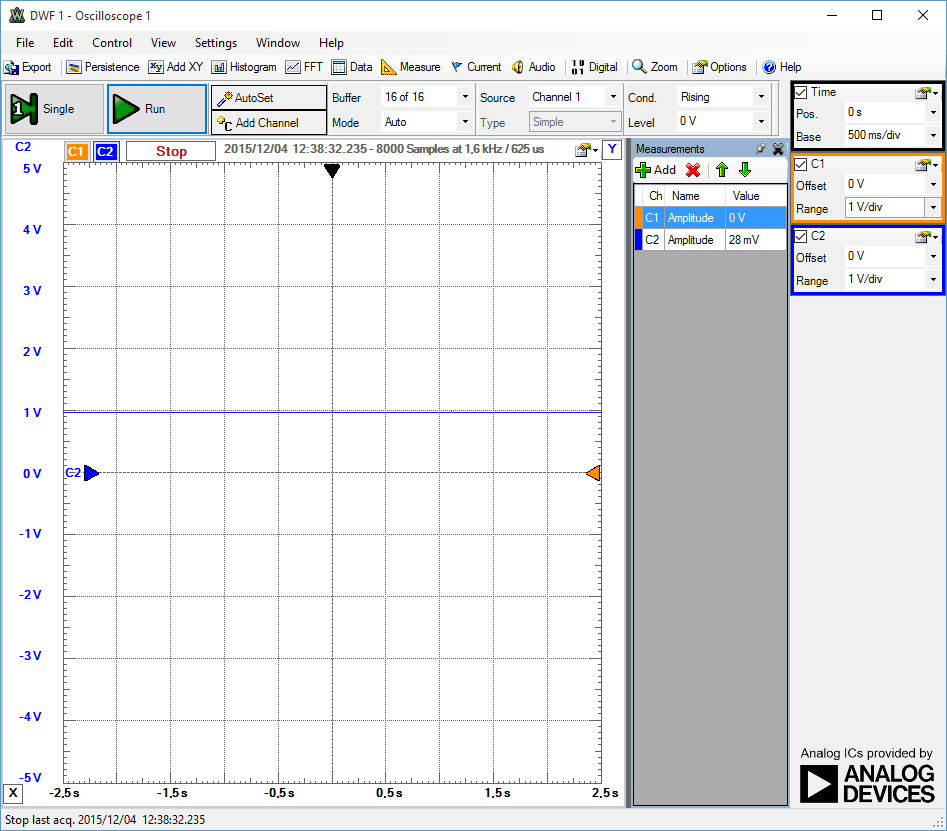
\includegraphics[width=0.6\textwidth]{Figurer/50mmhg}
	\caption{Måling ved 50 mmHg}
	\label{fig:vandtest_måling50}
\end{figure}
Ud fra figur \ref{fig:graf_vandtest} kendes udgangsspændingen også for de to andre målepunkter. Se under Modeltest i Dokumentationen for billeder af målingerne ved 10 mmHg og 100 mmHg. Målingen for 50 mmHg er her valgt ud, da denne måling ligger til baggrund for kalibreringen i softwaren. 

\section{Software}
\subsection{Design}
Overordnet set ønskes det at udvikle et system, der kan interagerer med en forsker. Diagrammet herunder viser at forskerens opgave består i at starte en måling, foretage en nulpunktsjustering og gemme de ønskede rådata, samt uafhængigt af systemet at bestemme en kalibreringskoefficient, hvis det ønskes. Diagrammet er en simpel illustration, som viser systemets adfærd gennem alle fem Use Cases. For yderligere præcisering af Use Cases se dokumentationen under Kravspecifikation. Formålet med dette diagram er at skabe et overblik over det samlede system. I de efterfølgende diagrammer dækker Transducer-blokken over alt hardware og DAQ'en. 
\begin{figure}[H]
	\centering
	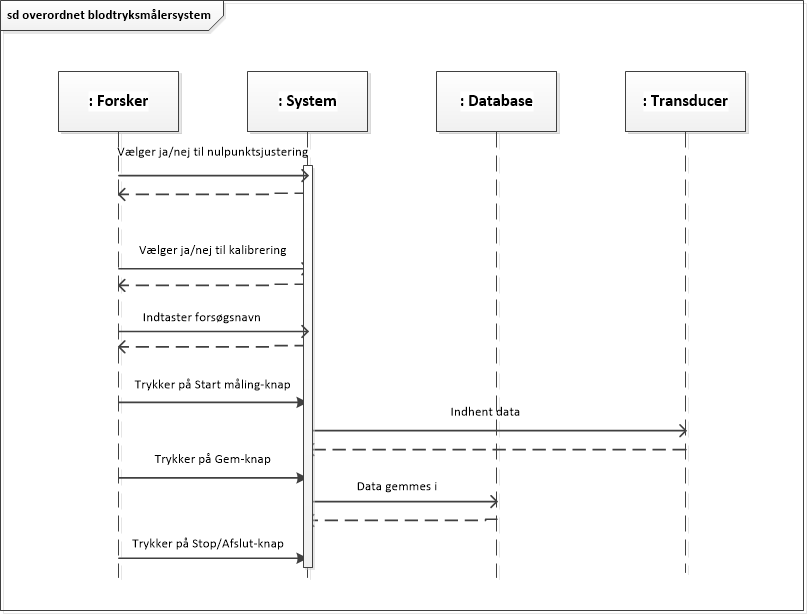
\includegraphics[width=0.7\textwidth]{Figurer/OverordnetSD}
	\caption{Overordnet sekvensdiagram for systemet}
	\label{fig:Overordnet sekvensdiagram}
\end{figure}

\subsubsection{Problemidentifikation}
Første step i softwaredesignet er at klarlægge, hvilke klasser systemet skal bestå af. Til dette er en domænemodel udarbejdet med udgangspunkt i de fem Use Cases. Modellen har til formål at vise, hvilke dele systemet skal holde styr på. Det ses at systemet primært vil centrere sig omkring selve den indhentede blodtryksmåling, da det er denne skal skal analyseres og bearbejdes. Samt omkring display hvorfra Forskeren får vist målingerne.  
\begin{figure}[H]
	\centering
	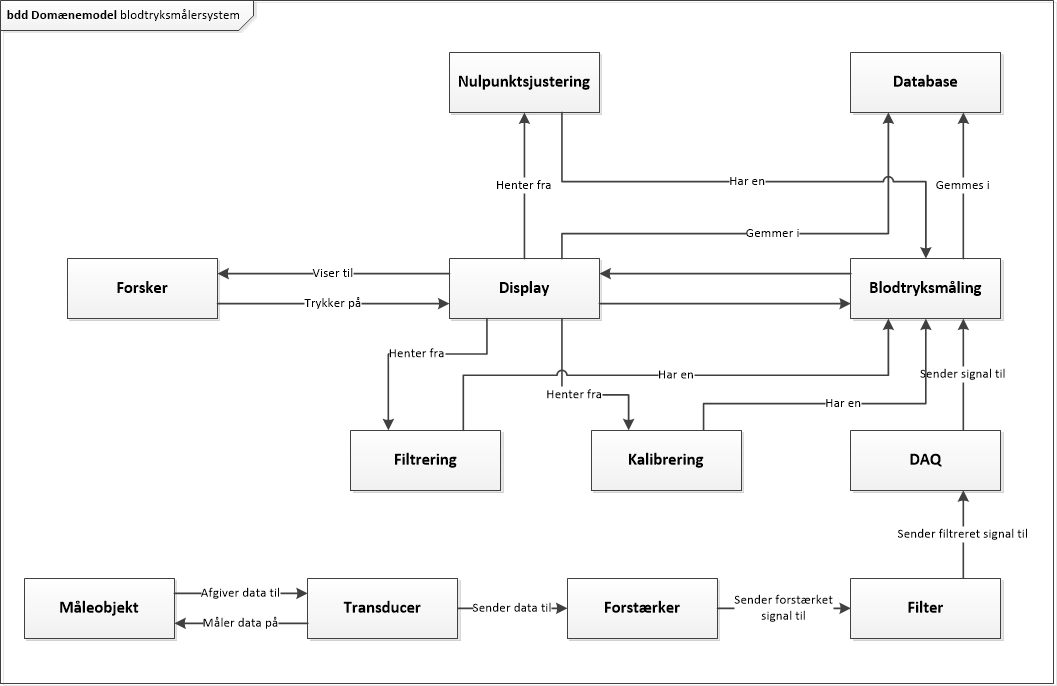
\includegraphics[width=1.0\textwidth]{Figurer/DomaneModel}
	\caption{Domænemodel}
	\label{fig:Domaenemodel}
\end{figure}
Analyse dækker over bestemmelse af systoliske, diastoliske og puls værdier. Hardwarekomponenterne er medtaget for at vise signalets vej fra måleobjekt til systemet. 

\subsubsection{Klasseidentifikation}
Domænemodel leder hen til udarbejdelse af en applikationsmodel. Denne model har til formål at vise hver enkelt klasses individuelle formål, samt hvilke domæne og boundary klasser der kommer i spil ved den pågældende Use Case. 
\begin{figure}[H]
	\centering
	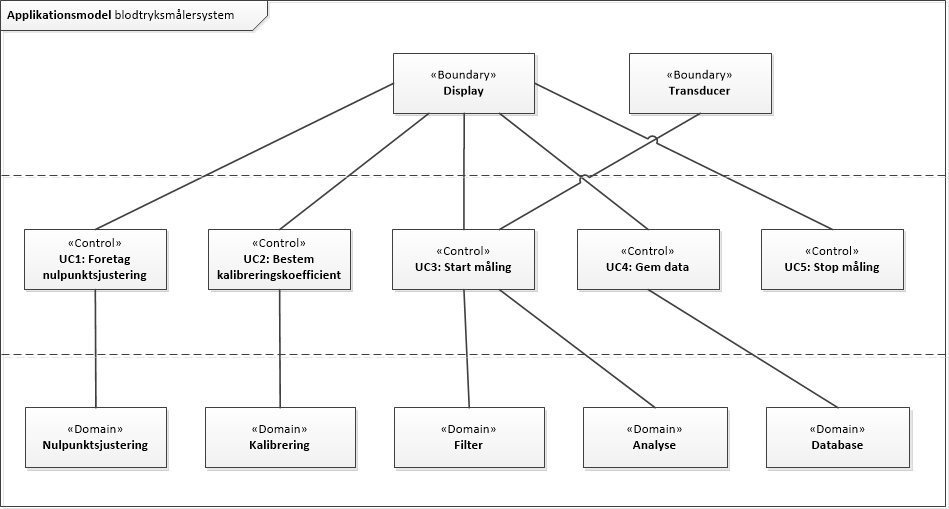
\includegraphics[width=1.0\textwidth]{Figurer/Applikationsmodel}
	\caption{Applikationsmodel for software}
	\label{fig:Applikationsmodellen}
\end{figure}
\subsubsection{Metodeidentifikation}
Klasserne i applikationsmodellen er med til at definere, hvilke blokke sekvensdiagrammer må indeholde. Dermed også med til at definere hvilke metoder i softwaresystemet, der er nødvendige for at få udført de ønskede handlinger mellem blokkene. Sekvensdiagrammer for hver enkelt Use Case kan ses i dokumenationen under Softwaredesign. 

\subsection{Implementering}
På baggrund af designfasen for softwaren kan implementeringen påbegyndes. Softwaredesignet viser at systemet skal implementeres med en GUI-applikation, hvor aktøren kan interagere med systemet. Derudover er det kendt at softwaren skal indeholde en række klasser, hvori funktionaliteter som kalibrering, nulpunktsjustering, digitalt filter og indhentning af systolisk, diastoliske og puls værdier skal placeres. I det følgende beskrives de overvejelser, der er gjort i forhold til implementering af disse funktionaliteter og softwaresystemet. 

Implementeringen af softwaren sker i Visual Studio 2013 i sproget C\#. Dette er valgt da programmet er et godt værktøj til at arbejde med GUI-applikationer, samt til håndtering af tråde og trådkommunikation. Tråde benyttes i softwaren da systemet, der skal implementeres, er et eventdrevet system. Det vil sige, at systemet skal kunne håndtere mange handlinger på en gang. Handlingerne igangsættes af events, der kommer af aktørens interaktion med systemet. Trådkommunikationen fungerer således, at en tråd kan sende et signal ud, som andre tråde kan reagere på.

\subsubsection{Klasse implementering}
På baggrund af designmodellerne er det besluttet at opbygge systemkoden efter principperne i en trelagsmodel\cite{3lagsmodel}. Trelagsmodellen indeholder et præsentations-lag, et logik-lag og et data-lag. Alt kommunikation i trelagsmodellen skal gå igennem logik-laget. Fordelen ved trelagsmodellen er, at den skaber et godt overblik i koden, og det fremstår tydeligt hvad hver enkelt klasses specifikke ansvar er. Et overordnet klassediagram over systemet er udarbejdet, se figur \ref{fig:KlassediagramSW}. Hvilke metoder hver enkelt klasse indeholder kan ses i Bilag under "Klassediagram". 
\begin{figure}[H]
	\centering
	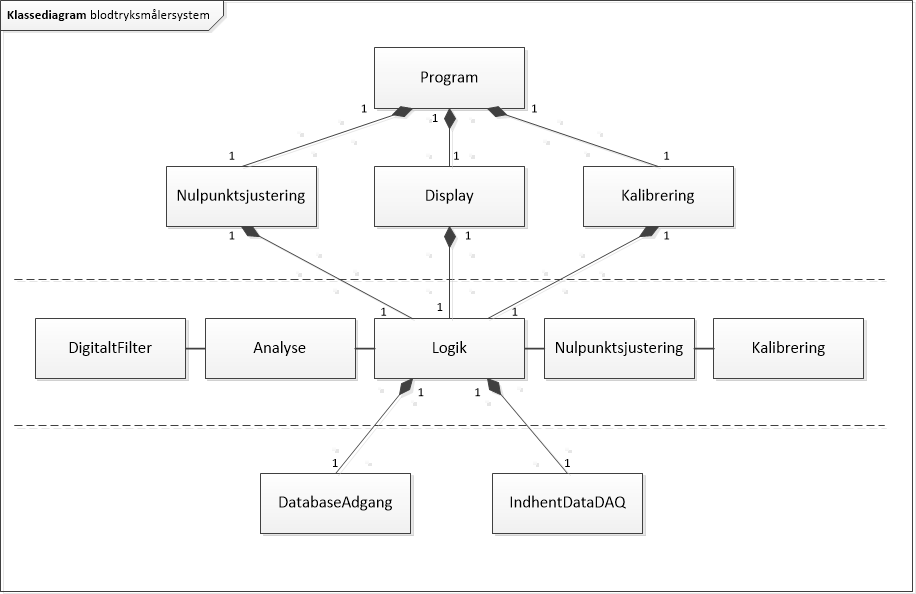
\includegraphics[width=1.0\textwidth]{Figurer/Klassediagram}
	\caption{Klassediagram}
	\label{fig:KlassediagramSW}
\end{figure}

\subsubsection{Brugergrænseflade}
Displayet (GUI) er Forskerens indgang til systemet. Derfor er det vigtigt at denne er opbygget efter forskerens logik. Til at klarlægge dette er principperne om en god brugergrænseflade taget i mente. \\
Det er et krav at Forsker indtaster et Forsøgsnavn inden en måling kan startes, derfor er komponenterne implementeres således at knappen Start Måling først bliver aktiveret, når Forsøgsnavn er indtastet i den tilhørende tekstboks. 
\begin{figure}[H]
	\centering
	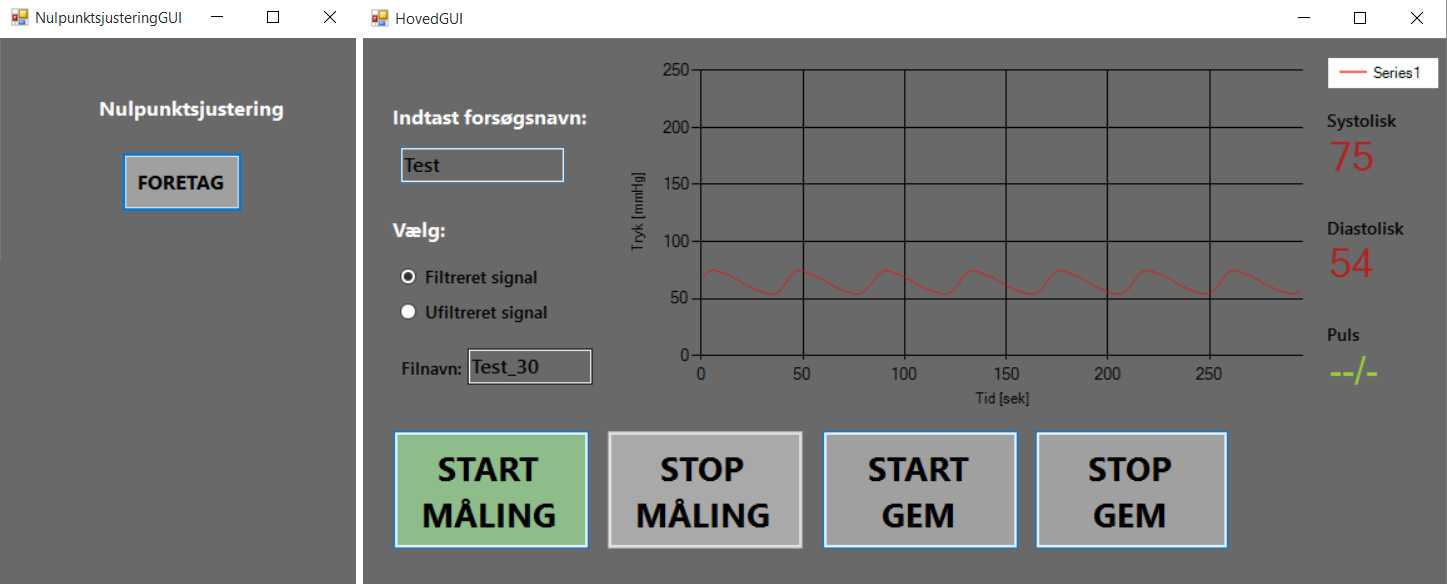
\includegraphics[width=1.0\textwidth]{Figurer/NulHovedGUI}
	\caption{NulpunktsjusteringGUI og HovedGUI}
	\label{fig:FormsSW}
\end{figure}
Af figur \ref{fig:FormsSW} ses det, at grafen er en væsentlig del af displays HovedGUI. Det vælges at få vist signalet i grafen, som en kurve. Førsteaksen indstilles til samples fra 0-300, og andenaksen til værdier fra 0-250 mmHg, hvilket er givet i kravspecifikationen. 

\subsubsection{Observer - Strategy}
Observer og Strategy er to programmeringsmønstre, det er valgt at opbygge softwarekoden efter. Grundet at de i samarbejde med hinanden er gode til, at håndtere en overførelse af data fra et lag til et andet. Observer definerer et "en til mange"\ relation mellem objekter således, at en ændring i et objekts tilstand medfører, at de mange objekter informeres om ændringer og dermed opdateres automatisk. Dette implementeres med to interfaces IObserver og ISubject. I disse interface er generelle metoder Notify(), Attach() og Gennemsnit() placeret, hvis ansvar er at flytte data fra en klasse til en anden, når metoden kaldes. Mønstret opbygges som en push.

Strategy mønstret indkapsler algoritmer og gør at metoder oprettet i interface kan overskrives i klasser der arver fra interfacet. Således at den nødvendige funktion kan tilføjes i den enkelt klasse.

Hvordan mønstrene er implemteret med relevante metoder kan skematisk ses i dokumantationen figur xx. I projektet blev mønstrene i første omgang benyttet fra logik-laget til præsentations-laget i forbindelse med at overføre data til visning i graf. Men undervejs viste det sig nødvendigt også at implementere mønstrene fra data-laget til logik-laget, således at det kan kontrolleres, hvor stor en mængde data, der sendes op af gangen. 

\subsubsection{Samplefrekvens}
Samplefrekvensen er som krav givet til 1000 Hertz. Hvilket svarer til at systemet modtager 1000 samples i sekunder. Varigheden af en sample er givet ved: 
\begin{ceqn}
\begin{equation}
\frac{1}{f_s}=\frac{1}{1000}=0.001 sek
\end{equation}
\end{ceqn}
Det har vist sig under arbejdet med softwaren, at grafen ikke kan følge med, når den modtager så mange målinger i sekundet. Derfor er det valgt at skære i antallet af målinger pr. sekund, der skal viderebearbejdes i logik-laget og udskrives i præsentations-laget. Antallet skæres ned til 50 målinger pr. sekund. Dette gøres ved at gennemsnittet af 20 målinger efter hinanden bestemmes, hvorefter gennemsnitsværdien returneres og gemmes i en liste, der sendes videre i systemet. Herefter findes gennemsnittet af de næste 20 målinger og således fortsætter det. 

\subsubsection{Nulpunktsjustering}
Formålet med en nulpunktsjustering er at flytte signalets offset op eller ned, så det atmosfæriske tryk altid er placeret ved 0 V på outputsignalet. Justeringsfaktoren er givet ved, hvor x er det målte atmosfæriske tryk i Volt modtaget gennem DAQ'en:
\begin{ceqn}
\begin{equation}
faktor_{jus}=0-(x)
\end{equation}
\end{ceqn}
Systemet ønskes nulpunktsjusteret for at sikre, at alle de målte blodtrykssignaler har samme udgangspunkt. Hvilket gør at målingerne kan sammenlignes. Systemet foretager nulpunktsjusteringen ved at retunerer gennemsnittet af de første 20 målinger fra DAQ'en, såfremt den tilsluttede transducer er åbnet så atmosfærisk tryk måles.  

\subsubsection{Kalibrering}
I dette projekt betyder kalibreringen, at kalibreringsfaktoren fra volt til millimeter kviksølv bestemmes. Denne bestemmes ved at tilkoble en væskesøjle til systemet. Væskesøjlen fyldes med vand til markering, så den vil give et kendt tryk (mmHg). Herefter kan output i volt fra hardwaren måles. Kalibreringskoefficienten er givet ved:
\begin{ceqn}
\begin{equation}
koef=\dfrac{x [mmHg]}{y [Volt]}
\end{equation}
\end{ceqn}
x angiver trykket fra væskesøjlen, denne hardcodes til 50 mmHg. Værdien for y angiver det målte spændingsoutput på hardwaren. Optimalt set er kalibreringskoefficienten 50.\\ 
Kaliberingen implementeres i softwaren ved brug af konfiguration. Forskeren beregner omsætningskoefficienten ud fra ligning 6.10. Resultatet af denne beregning indtaster Forsker i konfigurations XML-filen under App.settings. XML-filen kan tilgås uden opstart af systemet, derfor bliver kalibreringen uafhængig af, hvornår systemet kører og kalibreringen kan dermed foretages på et vilkårligt tidspunkt.

Det er vigtigt at pointere, at nulpunktsjusteringsfaktoren lægges til samtlige værdier i signalet før kalibreringskoefficienten ganges på. Dette udføres i kodens logik-lag.

\subsubsection{Digitalt Filter}
\cite{DSBsoft} Formålet med implementering af et digitalt filter er at fjerne støj fra det indhentede signal. Dette gøres ved at udglatte signalet. I projektet er det valgt at implementere et glidende middelværdifilter (moving average filter).\\ Fordelen ved dette filter er, at det er simpelt at forstå og det er optimalt at bruge på signaler i tidsdomænet.

Det glidende middelværdifilter fungerer ved midling af en række punkter fra inputsignalet for, at frembringe hvert punkt i outputsignalet. Hvilke punkter, der tages fra inputsignalet, vil flytte sig én plads for hvert beregnet outputpunkt, heraf kommer den glidende effekt. Matematisk er filteret givet ved:
\begin{ceqn}
\begin{equation}
y[i]=\frac{1}{M}\cdot\sum\limits_{j=0}^{M-1} x[i+j]
\end{equation}
\end{ceqn}
Hvor x[] er inputsignalet, y[] er outputsignalet og M er antallet af punkter, der benyttes i det glidende middelværdifilter. Denne beregning benytter sig udelukkende af punkter placeret på den samme side af output samplenummeret, hvilket vil føre til en relativ forskydning mellem input og output. M sættes til en længde på fem. Implementeringen af filteret er vist i et aktivitetsdiagram i dokumentationen under Software Implementering.\\
Filtret er implementeret således, at der minimum skal være 5 målinger i listen der skal filtreres førend, at filteret vil starte filtreringen. Dette er en begrænsning der ikke er optimal, men accepteres. Da den ikke vil være en begrænsning der vil påvirke Forskerens resultater i betydende grad. 

Systemet gør det muligt for Forsker at vælge på GUI om det filtrerede eller ufiltrerede signal ønskes udskrevet. 

\subsubsection{Analyse}
Analyse dækker over bestemmelsen af de systoliske, diastoliske og puls værdier ud fra blodtrykssignalet. Dette er implementeret i en klasse kaldet Analyse. I en blodtrykskurve er den systoliske værdi givet ved maksimum på kurven og den diastoliske er givet ved minimumsværdien på kurven. \\
Metoder hvori den maksimale værdi og den mindste værdi bestemmes er implementeret. Værdierne bestemmes ud fra listen der vises på grafen. Værdierne udskrives i labels på GUI. I præsentations-laget er implementeret en timer, der håndterer at de systoliske og diastoliske værdier på GUI opdateres hvert 3. sekund. Intervallet på 3 sekunder er valgt, da det er passende tid til at aflæse den pågældende værdi.

I forhold til implementering af puls er der gjort en række overvejelser om mulige løsninger. Puls er defineret ved slag pr. minut og på en pulsperiode vil der være en systole og diastole. Pulsen må derfor kunne bestemmes ved at tælle antallet af systoliske værdier på 6 sekunder. Antallet ganges med 10 for at få den rette enhed. En anden mulighed er også at bestemme pulsen ved at finde antallet af samples mellem to systoliske værdier. Omregnes samples til sekunder og ganges op til et minut, må dette være lig med Måleobjektets øjeblikkelige puls. Det er ikke lykkedes at implementere puls ved projektets aflevering.

\subsubsection{Database}
I systemet er der implementeret en lokal Database. Databasen er oprettet gennem hosten webhotel10.iha.dk. Formålet med Databasen er at lagre det målte blodtrykssignals rådata. Det er valgt at implementere Databasen af typen SQL, da denne database-type indeholder de funktioner, som er nødvendige for dette system. Data gemmes i tabeller i Databasen. Indledningsvis for at oprette den nødvendige tabel defineres en type til hver værdi. SQL-koden til oprettelse af tabel er vist på figur \ref{fig:SQL-kode}.
\begin{figure}[H]
	\centering
	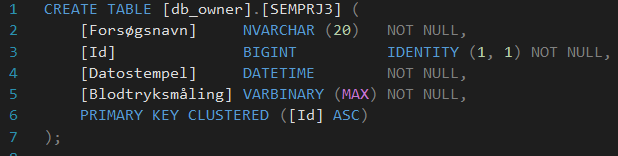
\includegraphics[width=0.7\textwidth]{Figurer/SQLDatabase}
	\caption{SQL-kode til oprettelse af tabeller i database}
	\label{fig:SQL-kode}
\end{figure}
For yderligere forklaring til de valgte SQL-typer, se dokumentationen under Software Implementering.

\subsection{Test}

\subsection{Integrationstest}
Til sidst i projekt forløbet blev en integrationstest udført. En integrationstest laves primært for at teste om softwaren fungerer korrekt og om enhederne/modulerne deri anvender hinanden. Testen retter sig mod afprøvning af det komplette program, med de eksterne systemer, i dette tilfælde sammen med hardwaren. 
Softwaren er langsomt blevet sammensat af de forskellige enheder som fremvisning af graf, indhentning af data, kalibrering, nulpunktsjustering, digitalt filter og at gemme. Hver gang én enhed har været færdig er den blevet testen, hvorefter en ny færdig enhed er blevet sat på osv. Tilsidst er der blevet udført  en test hvor alle enheder sættes sammen, software og hardware,  og der testes derpå. Testen kan sammenlignes med en ”Big Bang” test, da det var første kan vi satte den færdige software sammen med hardwaren.  
I dette tilfælde blev In Vitro maskinen i Cave Lab brugt til at skabe et blodtrykssignal. Dette blev sendt ind i vores system og sammenlignet med en anden ”rigtig” blodtryksmåler, som var tilkomplet samtidigt.  In vitro maskinen danner et tryk, som efterligner et hjerteslag.Trykket bliver skabt i vand, som presses igennem en falsk hjerteklap, derved er der opbygget en model af et hjerte som kan givet til blodtrykssignal. 
Billede af opstilling
Der startes med at laves en nulpunktsjustering på vores system, som bagefter viste en flot signal, som lå så konstant at det var svært at se cursoren. Samtidig stod systolisk- og diastolisktryk i tal på GUI. Her viste det sig, at vores system konstant afveg fra den anden blodtryksmåler med en værdi på 2, både på systolisk og diastolisk tryk. Da den konstant afveg, vurderes det at afvigelsen skyldes at vores sytem ikke var kalibreret eller at den anden blodtryksmåler ikke var nulpunktjusteret.  Der kunne ikke udføres en kaliberering da væskesøjlen var gået i stykker. Det blev også forsøgt at nulpunktjusterer den anden blodtryksmåler, men heller ikke dette kunne gøres.  Derfor blev resultatet af testen af vores system virker som det skal efter kravene stillet til det.  
Billeder af vores måling kontra den anden blodtryksmåler : gerne sammensat i et billede. 

\section{Resultater og diskussion}
Resultatet af dette projektforløb er blevet en prototype af en hardwaredel og et softwaresystem, hvis egenskab er at detektere den systoliske- og diastoliske værdi ud fra et blodtrykssignal. Denne prototype er blevet udviklet til forskningsbrug. Det kunne være en mulighed at videreudvikle systemet således, at det kan detektere hypotension og hypertension og så alarmere. På denne måde kunne systemet altså bruges til patientbrug, på hospitaler, sygehuse, lægehuse osv. \\
I starten af projektet var der stillet krav til både hardware- og softwaredelen, som alle er blevet opfyldt. Derudover er der blevet stillet nogle krav fra vejleder, som er forsøgt løst. Nogle er lykkes, andre er ikke (se problemrapport). Nogle af punkterne i accepttesten var ikke testbare, hvilket selvfølgelig bør opfyldes førend det ville være muligt at videreudvikle systemet. \\
I de ikke-funktionelle krav, var målsætningen en MTTR (Mean Time To Restore) på maksimalt 5 timer. Dette var ikke testbart, da systemet stadig var prototype og ikke et færdigt produkt.
Det tænkes ydermere, at det endelige produkts hardwaredele forefindes som en sammenkobling af alle dele, så forskeren kun skal styre en enkelt sammenkoblet hardware del, i stedet for fire dele (DAQ, Veroboard og to batterier). Det ville gøre det lettere for forskeren at styrer og transportere hardwaren og hvis nogle af delene i hardware skulle gå i stykker, ville det være nemt for forskeren blot at udskifte hele hardwaren, i stedet for at skulle fejlfinde og udskifte den bestemte del. Dette er selvfølgelig under forudsætningen af tilstedeværende reservedele - forsker vil altså kunne gendanne systemet indenfor 5 timer. \\
Da systemet stadig er en prototype, bestående af flere løse komponenter, der let kan frakobles, er risikoen for nedbrud relativt høj, hvilket ikke er optimalt for et færdigt produkt. En sammenkobling af alle løse komponenter, som nævnt før, skal sikre en længere Mean Time Between Failure. \\
Som projektformuleringen beskriver, er der udviklede en hardwaredel og et softwareprogram, der sammen kan detektere et blodtryk. Prototypen kan på under tre sekunder vise systolisk- og diastolisk blodtryk via en graf. Formålet og projektformuleringen er dermed blevet indfriet.  \\
Der er blevet arbejdet og designet en GUI, der i sidste ende har fået et relativt professionelt design, som vil være let, for en forsker, at benytte. Til videreudvikling vil det være nemt at implementere systemet, på f.eks. et sygehus, da de, som skal benytte systemet uden problemer vil kunne sætte sig ind i hvordan systemet håndteres. \\
Skal der påpeges en negativ ting om projektet og den endelige rapport, så må det siges at der har været en del forvirring omkring seta. Seta ønskes, for det meste, at være 1, hvilket der er blevet arbejde med i hele starten af projektet. Derfor var størrelserne på alle komponenterne bestemt ud fra en seta på 1. Fordi der arbejde med et 2. ordens butterworth sallen-key lavpasfilter, så er seta ikke 1, men 0,7. Dette var forvirrende og tog en del tid og forstå, hvorefter alle komponentstørrelserne skulle omregnes, så de passede til en seta på 0,7. Ved hardware har der derudover været en manglende forståelse for de signaler som sendes ind og måles ved udgangen. Det har givet en stor usikkerhed for, hvornår de forskellige blokke har virket korrekt. Derfor er der blevet spildt tid på at tro at systemet ikke virkede, mens det i virkeligheden gjorde som det skulle. \\
Ved softwaren er det specielt teorien bag tråde og derfor forståelsen derom, som har manglet og derved skabt flere problemer. Teorien for tråde skulle havde været i undervisningen, i kurset IT3, dette har dog ikke været fyldestgørende i forhold til brugen i projektet. \\
Kravene om kalibrering og nulpunktsjustering er også blevet opfyldt, selvom det volde mange problemer. Teorierne bag en kalibrering og en nulpunktsjustering var forståeligt, men hvordan det skulle fås til at fungere i en kode, var der ingen anelse om. Så det var problematisk at komme i gang med kodningen af disse. Derudover holde væskesøjle, som bruges til kalibrering, ikke særlig længe, så derefter blevet det ikke nemmere. 
I løbet af projektet er tidsplanen skredet adskillige gange. Blandt andet pga. mange uforudsete problemstillinger og udefrakommende faktorer, som f.eks. DSB-miniprojekter og en KSS-eksamen, der lå midt i det hele. \\

\section{Udviklingsværktøjer}
Gennem projektarbejdet har vi anvendt en række forskellige værktøjer til udvikling af blodtryksmåler-systemet. Disse er yderligere uddybet herunder.

\textbf{Visual Studio 2013}

Softwaredelen af projektets programmering er skrevet i sproget C-sharp. Her er Visual Studio 2013 anvendt som kompiler, da programmet gør det nemt at omskrive tekst til kode. Visual Studio 2013 indeholder også funktionen Windows Form Application, der visuelt kan fremstille de ønskede resultater i form af knapper, grafer og labels mv. i en samlet brugergrænseflade, som aktøren interagerer med. 

\textbf{Microsoft Visio 2016}

Microsoft Visio er et tegne værktøj, der i dette projekt er anvendt til at designe både SysML og UML diagrammer, som benyttes ved organisering af hardware og software design. Microsoft Visio er det oplagte valg, da diagrammer lavet i programmet får et enkelt og overskueligt udseende, og dermed fremstår det tydeligt for læseren hvad diagrammet vil vise.

\textbf{Analog Discovery og Waveform fra Digilent}

Analog Discovery og Waveform er i projektet benyttet som omformer og signal generator under testfasen. Her fungerer Analog Discovery som en Waveform generator, så et analog signal kan sendes videre ind i lavpasfiltret, forstærkeren og derefter ind i DAQ’en. I den endelig implementering erstattes Analog Discovery og Waveform med transduceren. 

\textbf{NI-DAQmx}

NI-DAQmx er et værktøj udarbejdet af National Instruments, som anvendes til at omforme det indkomne analoge signal fra transduceren (Analog Discovery) til et digital signal. Værdier fra NI-DAQmx er af en type som kan anvendes i selve softwarekoden. 

\textbf{\LaTeX}

\LaTeX\ er anvendt i projektet til design og opsætning af projektrapport og projektdokumentation. \LaTeX\ er god til tekstformatering, hvor opsætning og strukturer defineres samlet for hele rapport, samt god til versionsstyring. Til at skrive selve koden benyttes programmet TeX-maker som kompiler. 

\section{Opnåede erfaringer}
I dette projekt handlede det om, at integrere en hardware- og softwaredel. Derfor blev projektgruppen fra starten inddelt i en software og hardware gruppe, med indflydelse på hvilket område man ønskede at arbejde med. Ud over dette blev det aftalt hvem der stod for de praktiske ting, såsom mødeindkaldelser, mødereferater og tidsplan. Det gjorde at man i projektgruppen altid vidste, hvad der var blevet lavet og hvad de fremadrettede opgaver var. Det har gjort at tidsplanen er skrevet af en og at der derfor er en let forståeligt rød tråd igennem udviklingen af tidsplanen. At mødereferaterne kun er skrevet af en gør, at der har været en præcis skabelon, formatet og skriftsprog er det samme. Det samme kan siges om mødereferaterne. Det giver en bedre sammenhæng og en rød tråd igennem afsnittene.  
Selvom projektgruppen var delt i to, har grupperne altid siddet og arbejde sammen. På denne måde fik hele projektet en sammenhæng og en rød tråd igennem rapporten. \\
ISE blev brugt til udarbejdelse af dokumentation ved hjælp af diagrammer. Igennem projektet blev der i begge grupper, løbende lavet enhedstests og integrationstests i forbindelse med prototypen.\\
I hardwaredelen kunne der bruges erfaringerne fra fagene ASB og KVI, om hvordan forstærkning og filtre fungerer og bygges til det ønskede projekt. I faget KVI blev instrumentationsforstærkeren og strain gauges introduceret, hvorpå der kunne arbejdes videre med metoderne fra faget, hvilket har givet erfaringer til at bruge teorien i praksis, i form af projektet.\\
I softwaredelen blev der brugt erfaringerne fra 2. semesterprojekt ved bl.a. brug af tre-lags-modellen og oprettelse af en Database. Disse erfaringer er nu blevet udvidet til at bruge tråde ved indsamling af data og en kontinuerlig visning i en graf. Ligeledes er Observer-Strategy princippet og nye algoritmer til udskrivelse af systolisk- og diastolisk værdi, nu en del af koden. Der er et digitalt filter i softwaren, hvorfra viden og erfaringer fra DSB er blevet brugt til at opsætte sampling, aliasering og filter.\\
Underviserne har været enormt behjælpelige, hvilket har aflastet projektvejlederen, således at møderne kunne blive afholdt væsentlig mere effektivt, og det har givet et detaljeret og præcist svar, at snakke med underviseren der har undervist i det fag, der har volt problemer, da det ikke kan forventes af vejlederen, at have styr på det hele. \\
I dette semester blev det valgt at skrive rapporten og dokumentationen i \LaTeX, som var nyt for de fleste. Dette har voldt utrolig mange problemer og frustrationer.  Der er blevet arbejdet særdeles meget med dette skriveprogram og der har flere gang været gruppemedlemmer, der har haft lyst til at slå en knytnæve igennem deres computerskærme, men til sidst har alle kunne se fordelene ved at benytte \LaTeX som skriveprogram. Det ser virkelig professionelt ud og det er lækkert at billeder og figurer ikke hopper rundt, som de f.eks. gør i skriveprogrammet Word. Derfor har alle i semestergruppen været glade for valget af \LaTeX. \\


\section{Perspektivering - Fremtidigt arbejde}
I fremtiden vil blodtryksmåleren kunne udvides gennem flere muligheder. Da blodtryksmåleren er lavet til forskningsbrug, har der i projektforløbet ikke været nogle idéer til at udvikle den til patientbrug. Dette er dog ikke umuligt, da alle grundprincipperne omkring en god blodtryksmåler er opfyldt, og der ville kunne arbejdes på usability til sygeplejeskerne. Softwaren skal også opdateres til patientjounaler og lign. Men igen, er det overhovedet ikke umuligt at optimere blodtryksmåleren til patientbrug. Det vil her være en god idé også at lave en alarm til blodtryksmåleren, som viser når blodtrykket er for lavt/højt. En anden forlængelse af systemet kunne være en metode, som skal kunne vise gemte målinger. Dette vil være nyttigt hos både forskere og til en udvidet patient-blodtryksmåler, da det skaber overblik og perspektiv for forskeren/lægen. \newline Et log-in vindue er en anden ting, som kunne forbedre systemet, for på den måde at skabe større sikkerhed for forskeren og dataene. Et log-in vindue vil gøre at en forsker kan være sikker på, at hans målinger og forskning ikke kan tilgås af andre. Dette kræver en større udvidelse, hvor der skal laves et log-in vindue og en database, hvor password og brugernavn gemmes. Der skal også laves en metode, som kan tjekke om det indtastede password og brugernavn passer over ens med det i databasen. 
\newline
Generelt skal de standarter, som findes for blodtryksmålere undersøges grundigere. Specielt brugergrænsefladen, men også resten af systemet som enheder og visning af graf, skal rettes til efter de passende standarter.
\newline 
Hvis systemet ydeligere skulle tilpasses forskning, kunne det gøres gennem en bedre navngivning af data i tabellen eller et bedre overblik over, hvordan data bliver gemt f.eks. gennem en liste for de gemte målinger. På den måde vil det blive nemmere for forskeren at finde frem til gamle målinger.
I fremtidigt arbejde skal systemet også være i stand til at vægte de enkelte værdier som fås i blodtryksmåleren. Dette betyder at systemet skal kunne vurdere integriteten af tallene, og se hvilket tal der skal lægges mest vægt på, ud af de fem, som derefter summeres, for at give en.   
\newline 
I forhold til hardware er målet, at det hele skal samles i en kasse. Så det på den måde ikke er muligt at ændre eller stille ved det. Derved skal filteret og forstærkningen laves på en printplade. Samtidigt skal det ved kassen være en plads til batterierne, hvor det er muligt at kunne skifte dem, når nødvendigt. Derved fås et samlet system, som nemt kan flyttes rundt på og som ikke er i fare for at gå i stykker. Dette system kan også, i stedet for udskiftelige batterier, have et genopladeligt lithiumbatteri, som vil kunne lætte besværet ved ofte at udskifte batterier.